% !TEX root = ../paper.tex
\section{Results and Examples}

\subsection{Forge as a Lean DSL}\label{sec:dsl}
One of the crucial benefits of working with Lean 4 as a metaprogramming language and a target for our translation is the rich support for domain-specific language (DSL) implementation and integration. Lean and its accompanying Language Server Protocol (LSP)\footnote{This is the language server that processes Lean code and communicates with the code editor or integrated development environment. In this case, we use VS Code.} are designed to have highly flexible and extensible user interfaces that expose useful APIs for implementers of DSLs and custom UI to utilize \cite{moura2021lean, nawrocki2023extensible}. Furthermore, Lean's extensible syntax and macro system are simple yet remarkably powerful \cite{ullrich2022beyond, metaprogramming}. 

It is as such that we justify framing our implementation of Forge in Lean as a domain-specific language (DSL). We do not treat user experience of our tool as an afterthought, nor do we skimp over ensuring that \textsc{Lforge} has a set of developer tools just as capable as those found in Forge or Lean themselves. As mentioned in \cref{sec:design-summary}, the fact that we can interact with Lean's implementation means that many of Lean's `IDE-like' features are exposed to us and available for us to use in the Forge DSL without much overhead. 

The following are some (non-exhaustive) examples of the user experience and interface of Forge within Lean. Code examples are taken from the example specifications described in \cref{appendix:additional-examples}. 

\subsubsection{Syntax Highlighting}

Superficially, by defining our syntax as Lean objects and isolating our keywords (we piggyback off Lean's lexer), we get syntax highlighting of Forge code `for free', on par with Forge's native VS Code extension solutions. In \cref{fig:sc-highlighting-hover}, the syntax of a Forge specification is color-coded. 

\subsubsection{Types on Hover}

Lean exposes an \texttt{addTermInfo'} method that allows us to attach declared names to pieces of syntax (nodes in Lean's concrete syntax tree), including custom syntax like ours for Forge. As such, we can annotate relevant pieces of syntax within our Forge specification to reflect names and types that are within scope. When the user hovers their cursor over a piece of syntax corresponding to a Forge expression, a hovering tooltip will display the type of the expression. In \cref{fig:sc-highlighting-hover}, the tooltip shows the type of a Forge predicate defined earlier in the file. 

\begin{figure}
  \centering
  \fbox{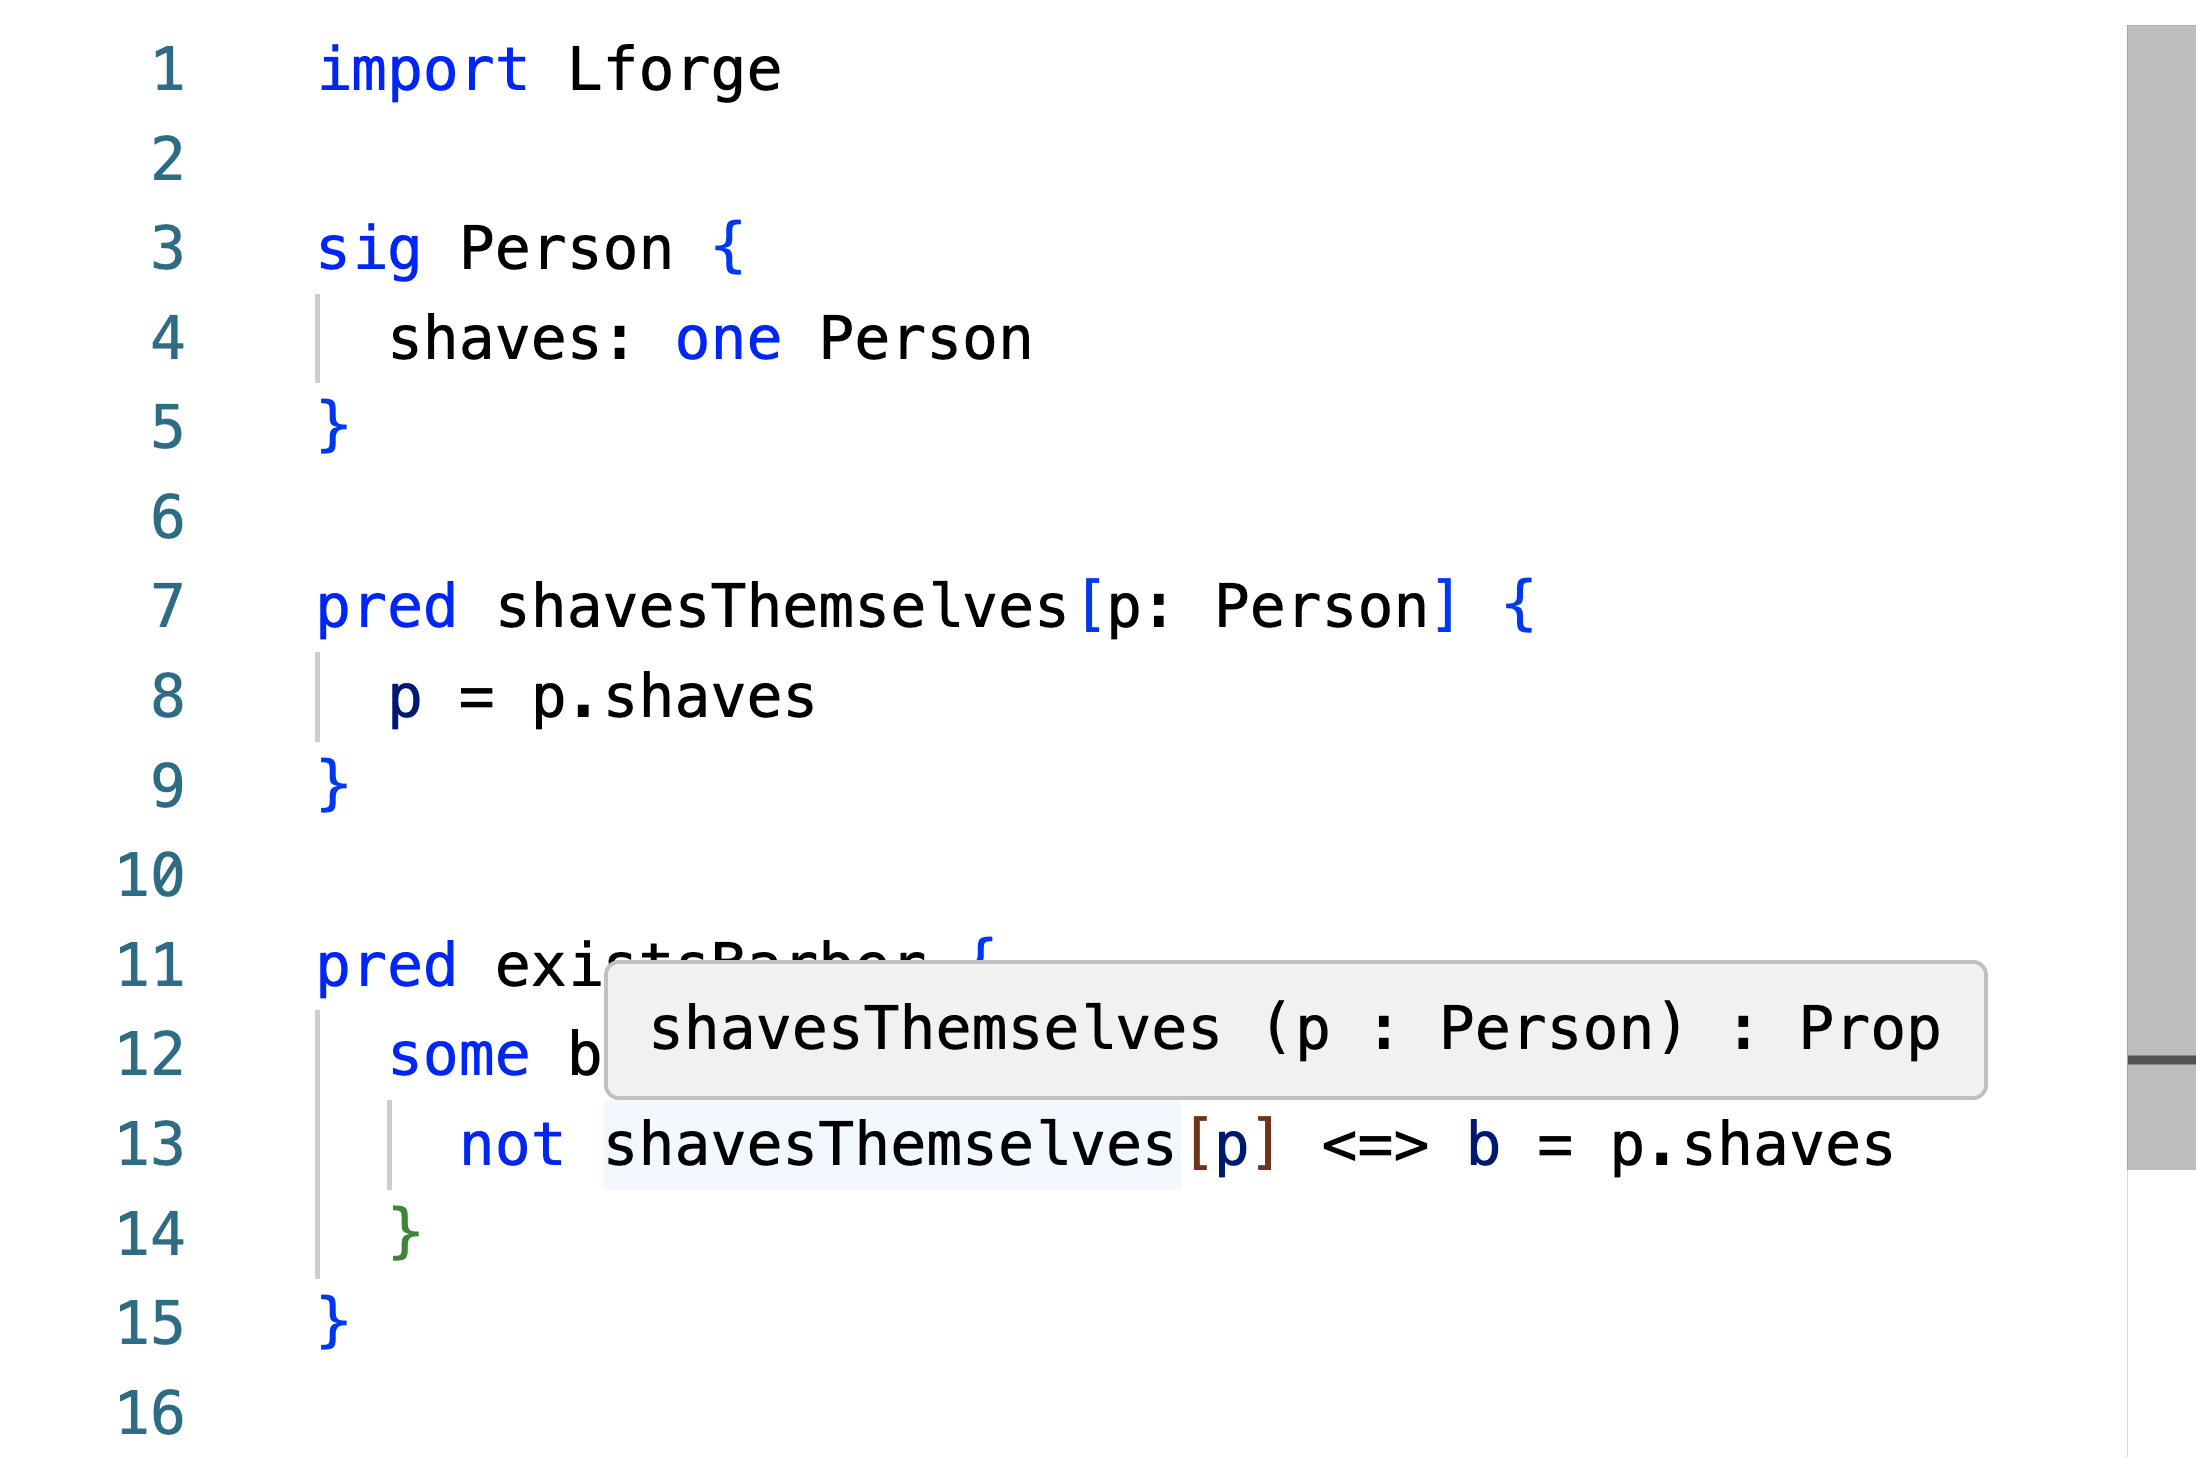
\includegraphics[width=0.5\textwidth,trim={0 0 0 0},clip]{images/screenshots/hover-tooltip.png}}
  \caption{Tooltips containing type information are available on hover. Forge syntax is automatically highlighted without any extra work.}
  \label{fig:sc-highlighting-hover}
\end{figure}

\begin{figure}
  \begin{center}
    \fbox{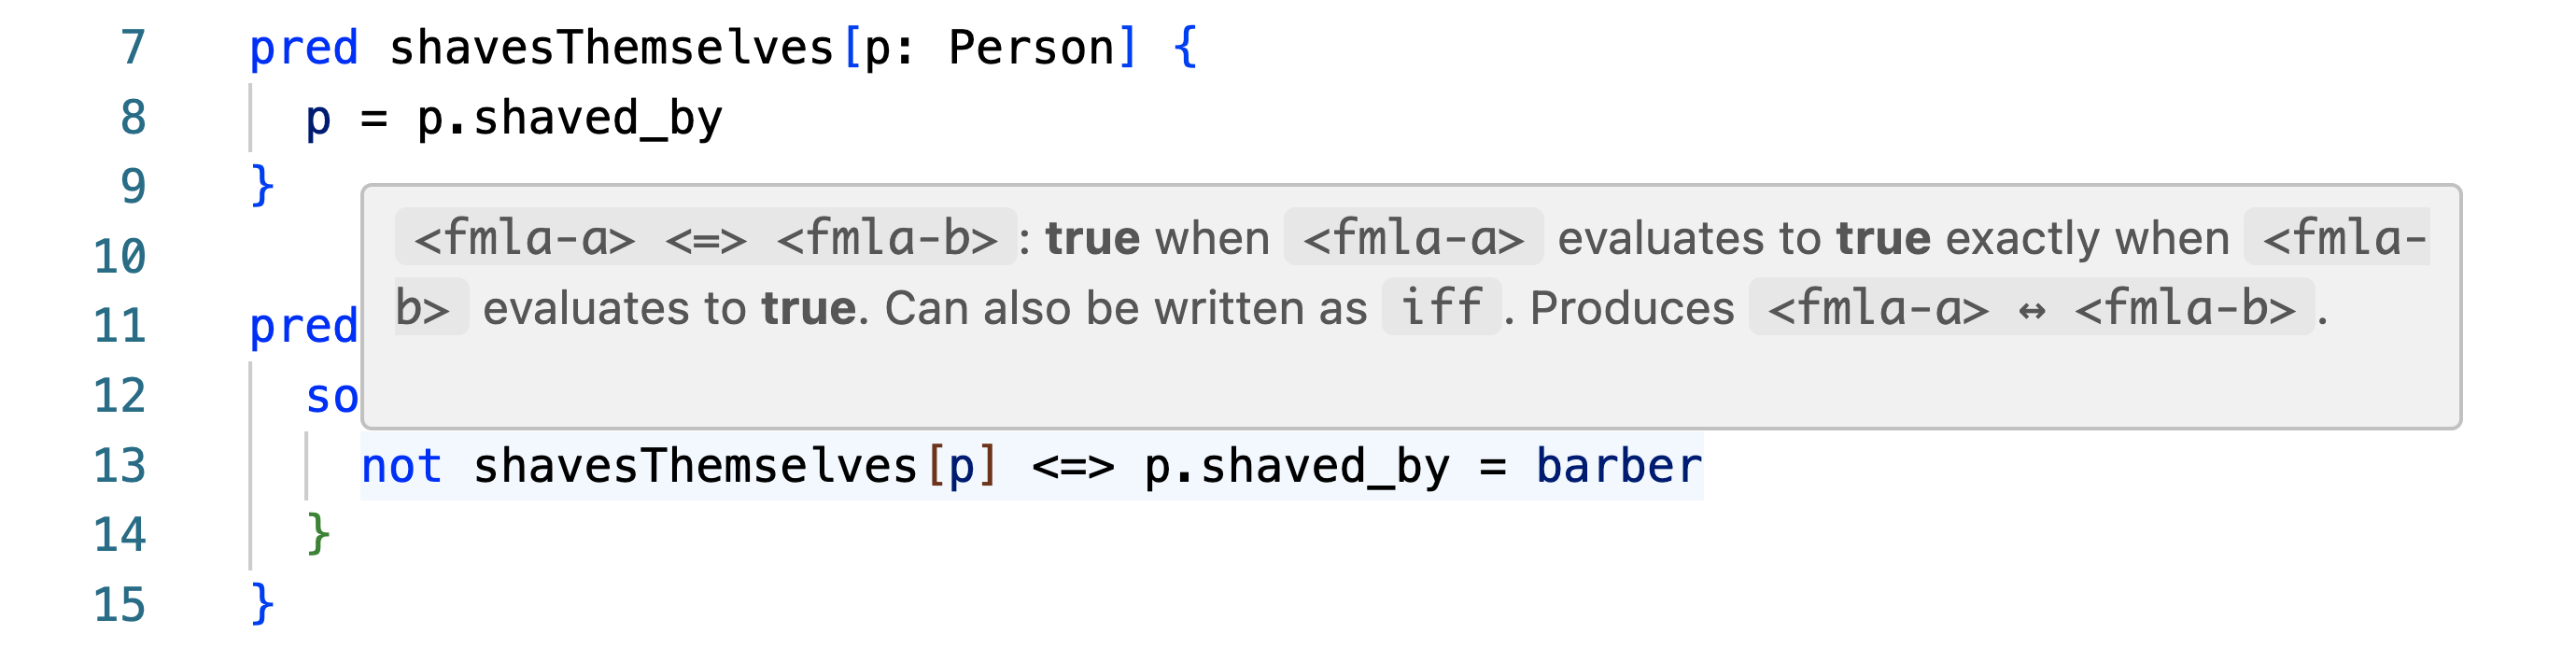
\includegraphics[width=0.7\textwidth,trim={0 0 0 0},clip]{images/screenshots/documentation.png}}
  \end{center}
  \begin{center}
    \centering\fbox{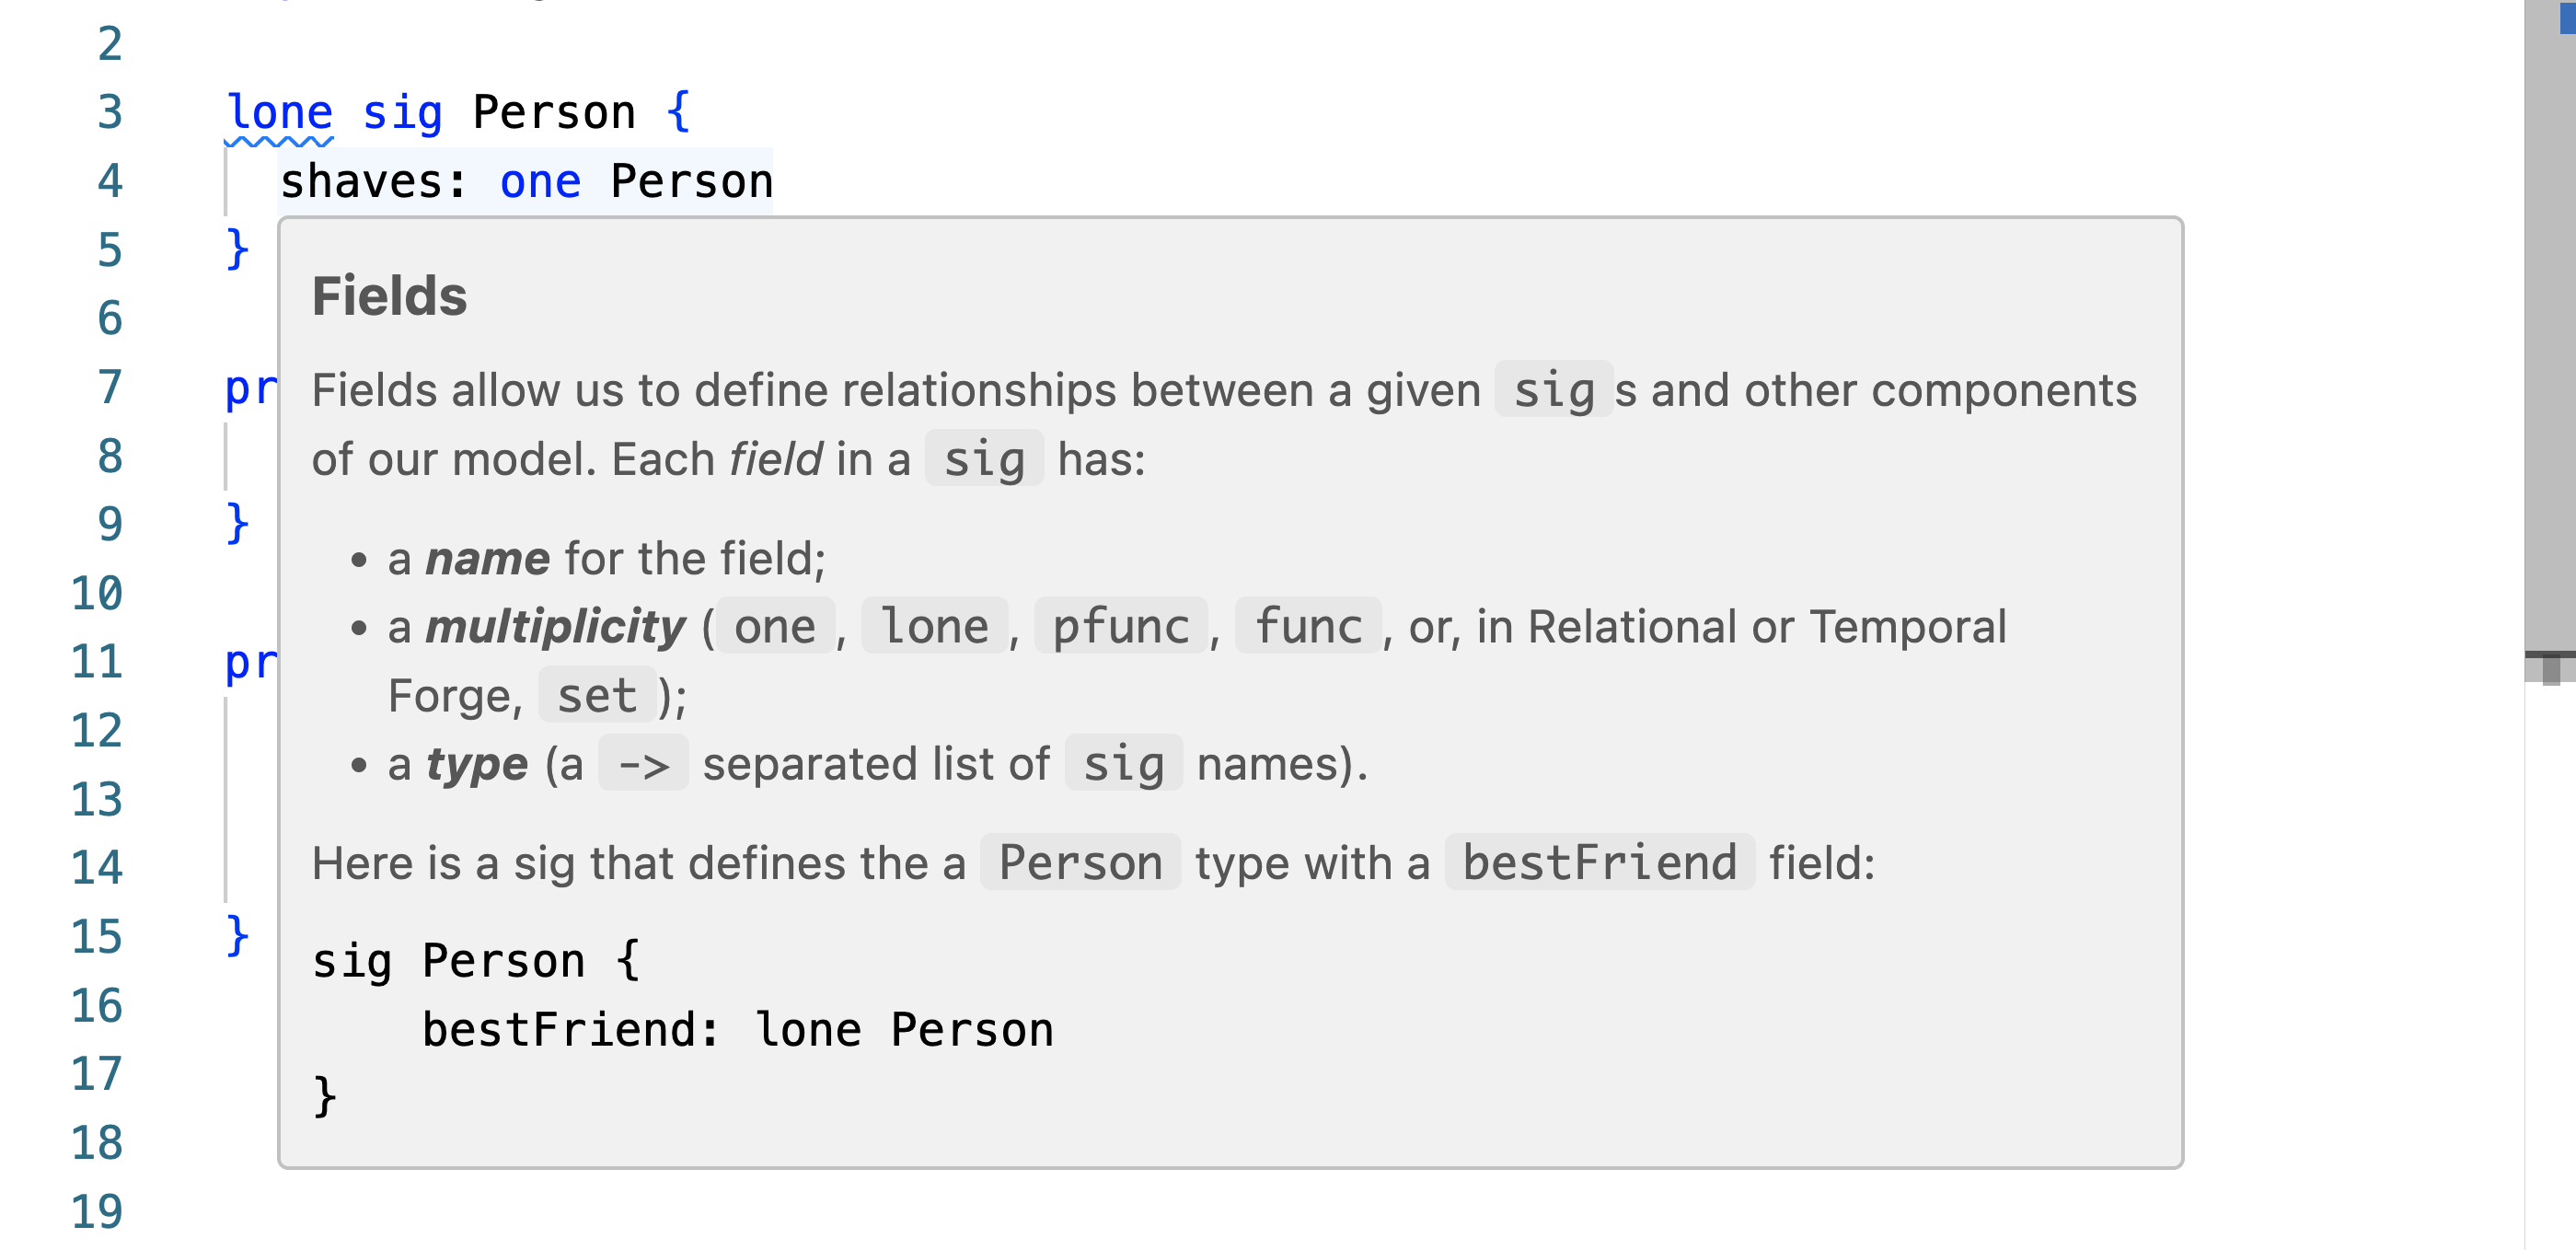
\includegraphics[width=0.7\textwidth,trim={0 0 0 0},clip]{images/screenshots/documentation-fields.png}}
  \end{center}
  \caption{We can define our syntax definitions to print with custom documentation text for users new to using Forge syntax. }
  \label{fig:sc-docstrings}
\end{figure}

\subsubsection{Documentation}

As a pedagogical language, Forge has a focus on usability, learnability, and helpful feedback \cite{ngpdbccdlrrvwwk-oopsla-2024}, especially when its parent language Alloy is far more permissive and obscure with errors. We follow in the same vein in reporting errors and missing features, and, in addition, we include documentation on Forge's syntax through on-hover features. 

Forge documentation is included via docstrings that are placed inline with our syntax objects (see \cref{sec:parsing}), which is automatically included by Lean's LSP to display on the front end. \Cref{fig:sc-docstrings} showcases docstrings of varying verbosity for operators as well as declaration syntax. 

Additionally, we need to be clear and verbose about language features that are not supported in \textsc{Lforge}. Since \textsc{Lforge} includes a subset of relational Forge determined by compatibility with Lean's semantics, we prompt users attempting to use unsupported language features with clarification and a request to redefine their statements. \Cref{fig:sc-unsupported} showcases an example of a prompt that \texttt{lone} sig quantifier is unsupported and potentially ambiguous. 

\begin{figure}[h!]
  \centering
  \fbox{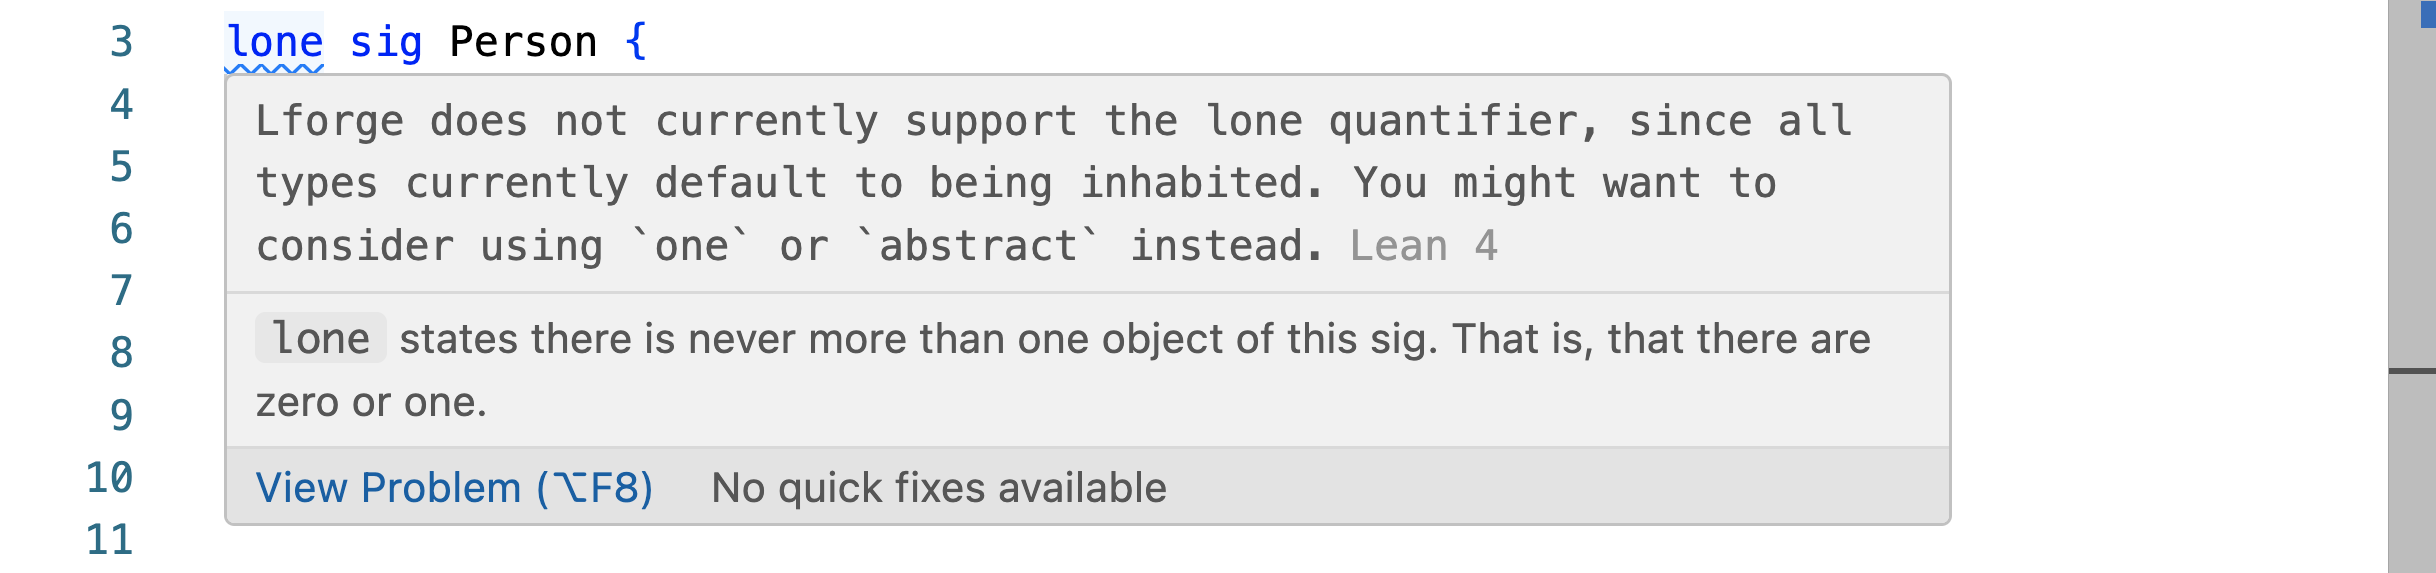
\includegraphics[width=0.7\textwidth,trim={0 0 6cm 0},clip]{images/screenshots/custom-errors.png}}
  \caption{We can define custom error messages with our implementation to prompt users to change their specifications if a piece of syntax is ambiguous or not supported.}
  \label{fig:sc-unsupported}
\end{figure}

\subsubsection{Error Checking}

Compared to Forge or Racket, Lean (and consequently, \textsc{Lforge}) provides a markedly better experience with error messages and prompting users when there are errors present in their source program. Since Lean runs in the background as an LSP, users get immediate feedback on whether their source code parses and `compiles'.\footnote{Forge translations in Lean are not executable, so they provide their value in being interactive with the proof system.}

Lean's error locality system allows its error monad to refer to any piece of syntax object to potentially throw an error. This allows us to prompt errors as soon and as granularly as possible. \Cref{fig:sc-type-mismatch} illustrates error reporting at the level of specific identifiers. 

\subsubsection{Types}

Lean's dependent type system is both a blessing and a curse when it comes to the task of translating a language with a foreign type system into Lean. While the elaborator is a highly optimized algorithm that attempts to resolve type coercions, type classes, and reductions \cite{de2015lean}, it is often delicate and temperamental, especially when we are working at such a low level of emitting Lean \texttt{expr}s, which happens \emph{after} type unification (see \cref{sec:elaboration}). We discuss some of the downsides of such a strict type system in \cref{sec:type-coercions}, and introduced \textsc{Lforge} features that circumvent Lean's restrictions and play into Lean's type system. 

Here, we discuss some of the merits of implementing a DSL designed around Lean's extensive type system. One of the side effects of translating Forge into Lean is that we inherit Lean's powerful type unification and checking system. This allows us, at specification-time, to check for type errors within the specification. Alloy, on the other hand, is purposefully untyped \cite{jackson2019alloy}\footnote{Whether or not they should be is discussed in \cite{lamport1999should}. We believe that there can be a reasonable compromise that allows type systems to be useful aids for students and users. } and only reports type errors at runtime when the successful evaluation of expressions results in the empty expression \cite{edwards2004type}. This proves difficult to debug and unwieldy for users to understand, as \cite{ngpdbccdlrrvwwk-oopsla-2024} observes. For students who are newly learning the idea of relations, sets, and units, instantaneous feedback on the validity of types and expressions is immensely useful. 

Since expressions in our Forge DSL need to translate to typed terms in Lean, we necessarily have to specify types (or use Lean metavariables awaiting unification in place of types) to the Lean expressions emitted. Fortunately, much of this process is abstracted away by the type inference system in place in Lean. For example, to make an application, say, a set union, we don't need to specify the type of set that is being used in the operands and \texttt{mkAppM} will complete that for us. However, if we specified two sets of different types, Lean would raise an error. This results in a type-checking and inference system that is as powerful as Lean's with minimal overhead. 

Since the Lean LSP provides type error and linting, our Forge DSL inherits this feature as well. In \cref{fig:sc-type-mismatch}, we pass the \texttt{Board} and \texttt{Player} arguments to \texttt{winRow} in the wrong order, which causes a type error. Lean can identify that the first input to \texttt{winRow}, \texttt{p}, has the wrong type and displays an appropriate error message. 

\begin{figure}[h!]
  \centering
  \fbox{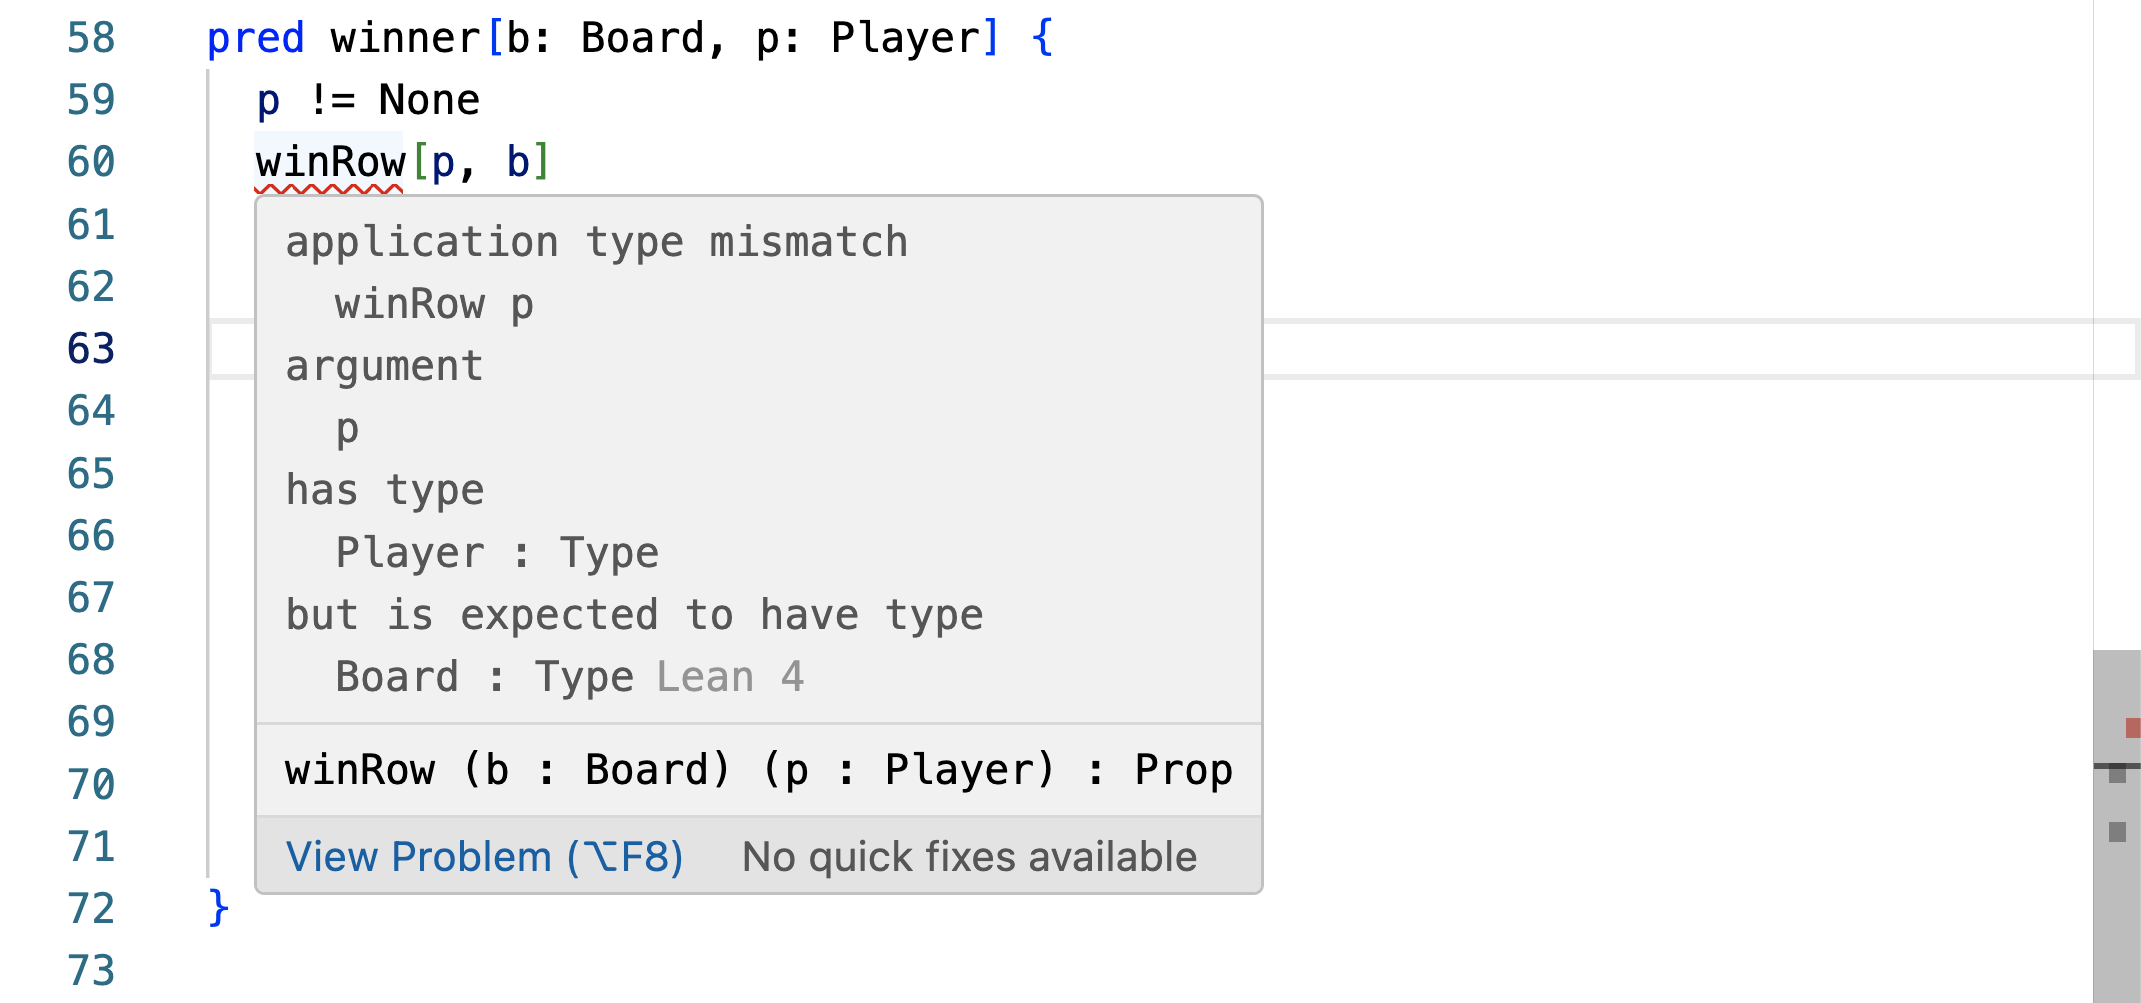
\includegraphics[width=0.6\textwidth,trim={0 0 0 0},clip]{images/screenshots/type-check.png}}
  \caption{A Lean error message indicating a type mismatch in our Forge expression.}
  \label{fig:sc-type-mismatch}
\end{figure}

\subsubsection{Mixed Specification}

Our embedding of Forge within Lean, especially our choice to map Forge structures (sigs, fields, predicates) to corresponding Lean concepts (types, relations, functions) as faithfully as possible means that a Lean file with Forge specifications supports mixed specification, an embedding model similar to those explored and supported by similar tools that merge the Alloy specification into other imperative programming languages \cite{milicevic2010executable,milicevic2014alpha,milicevic2015advancing}. 

All Forge specifications, once inserted into a Lean file, will generate appropriate definitions directly into the Lean environment. Using Lean syntax, we can further interact with these definitions from Forge, perhaps writing predicates or definitions that build on these. This interaction goes the opposite way as well: where Forge expects an expression, predicate, or function, declarations from Lean can be used seamlessly. This provides a frictionless user experience and allows the user to add additional constraints and rules, written in Lean, to a preexisting Forge model. 

For example, Forge does not support recursive predicates and functions, and current paradigms involve adding helper fields to aid in keeping track of recursive values, like the depth of a tree. While in Lean, a recursive \texttt{depth} function would be easy to implement and produce proofs around. 

Furthermore, this alleviates the tension incurred in creating the perfect translation: we are aware of the fact that only a subset of Forge is implemented due to the technical restrictions of both platforms. However, with appropriate error reporting (see above Error Checking), users can be prompted to extend their Forge specifications with additional Lean rules. Mixed specification of Forge and Lean means that Forge specifications are now extensible using a much broader functional programming language. 

The following is an example of mixed specification of Forge and Lean using \textsc{Lforge}. The full specification of this example, a model for mutual exclusion of processes, is discussed in \cref{sec:mutex}. 

% !TEX root = ../../paper.tex

{
\setlength{\fboxsep}{4pt}
\begin{tcolorbox}[listing only, minted style=autumn, colback=forgelistingcolor, enhanced, frame hidden, top=0pt, bottom=0pt, left=0pt, right=0pt]
\vspace{-0.5em}
\begin{minted}[bgcolor=leanlistingcolor,linenos,frame=none,firstnumber=1]{lean}
import Lforge
\end{minted}
\vspace{-3.7em}
\begin{minted}[bgcolor=forgelistingcolor,linenos,frame=none,firstnumber=2]{alloy}

abstract sig Location {}
one sig Uninterested, Waiting, InCS extends Location {}

sig Process {}

sig State {
  loc: func Process -> Location,
  flags: set Process
}

\end{minted}
\vspace{-3.7em}
\begin{minted}[bgcolor=leanlistingcolor,linenos,frame=none,firstnumber=13]{lean}
def flags_good (s : State) :=
  ∀ (p : Process), loc s p = InCS ∨ loc s p = Waiting → flags s p
\end{minted}
\vspace{-3.7em}
\begin{minted}[bgcolor=forgelistingcolor,linenos,frame=none,firstnumber=15]{alloy}

pred good[s: State] {
  flags_good[s]
  lone {p: Process | s.loc[p] = InCS}
}
\end{minted}
\vspace{-2em}
\end{tcolorbox}
}


While the majority of this specification is in Forge, we are working in Lean using \textsc{Lforge} (line 1). We define relevant sigs and fields as a Forge specification. On lines 13-14, we use the types defined in Forge to write a predicate in Lean that states that all processes waiting or in a critical state have a flag raised. In line 17, we've switched back to specifying in Forge but can continue to utilize the \texttt{flags\_good} predicates we wrote above in Lean. There are no walls or abstractions between the two languages, and Forge inhabits the Lean environment as a first-class citizen. 

Since this interoperability works across imports and modules, we envision projects where sections of specifications can be written in Forge and other relevant sections in Lean, allowing users to interoperate between the two. This could also introduce possibilities for users accustomed to the two distinct languages or formalization techniques to collaborate on a shared specification. 

\subsection{A Toy Example, \emph{Continued}}\label{sec:toy-example-continued}

We revisit our toy example from \cref{sec:toy-example} (the barber who ``shaves all those, and only those, who do not shave themselves''). Recall that we had introduced a Forge specification for this problem, as well as an equivalent Lean specification of the paradox. We concluded earlier that while it was insightful for Forge to produce a result that this specification was \texttt{Unsatisfiable}, we might still desire a general proof of this fact outside of Forge's finite and restricted search bounds. 

In \cref{fig:barber-proof} below is an example of what the last part of the modeling workflow---writing and completing the proof---would look like in Lean's interactive tactic mode: 

\begin{figure}[h!]
  \centering
  \fbox{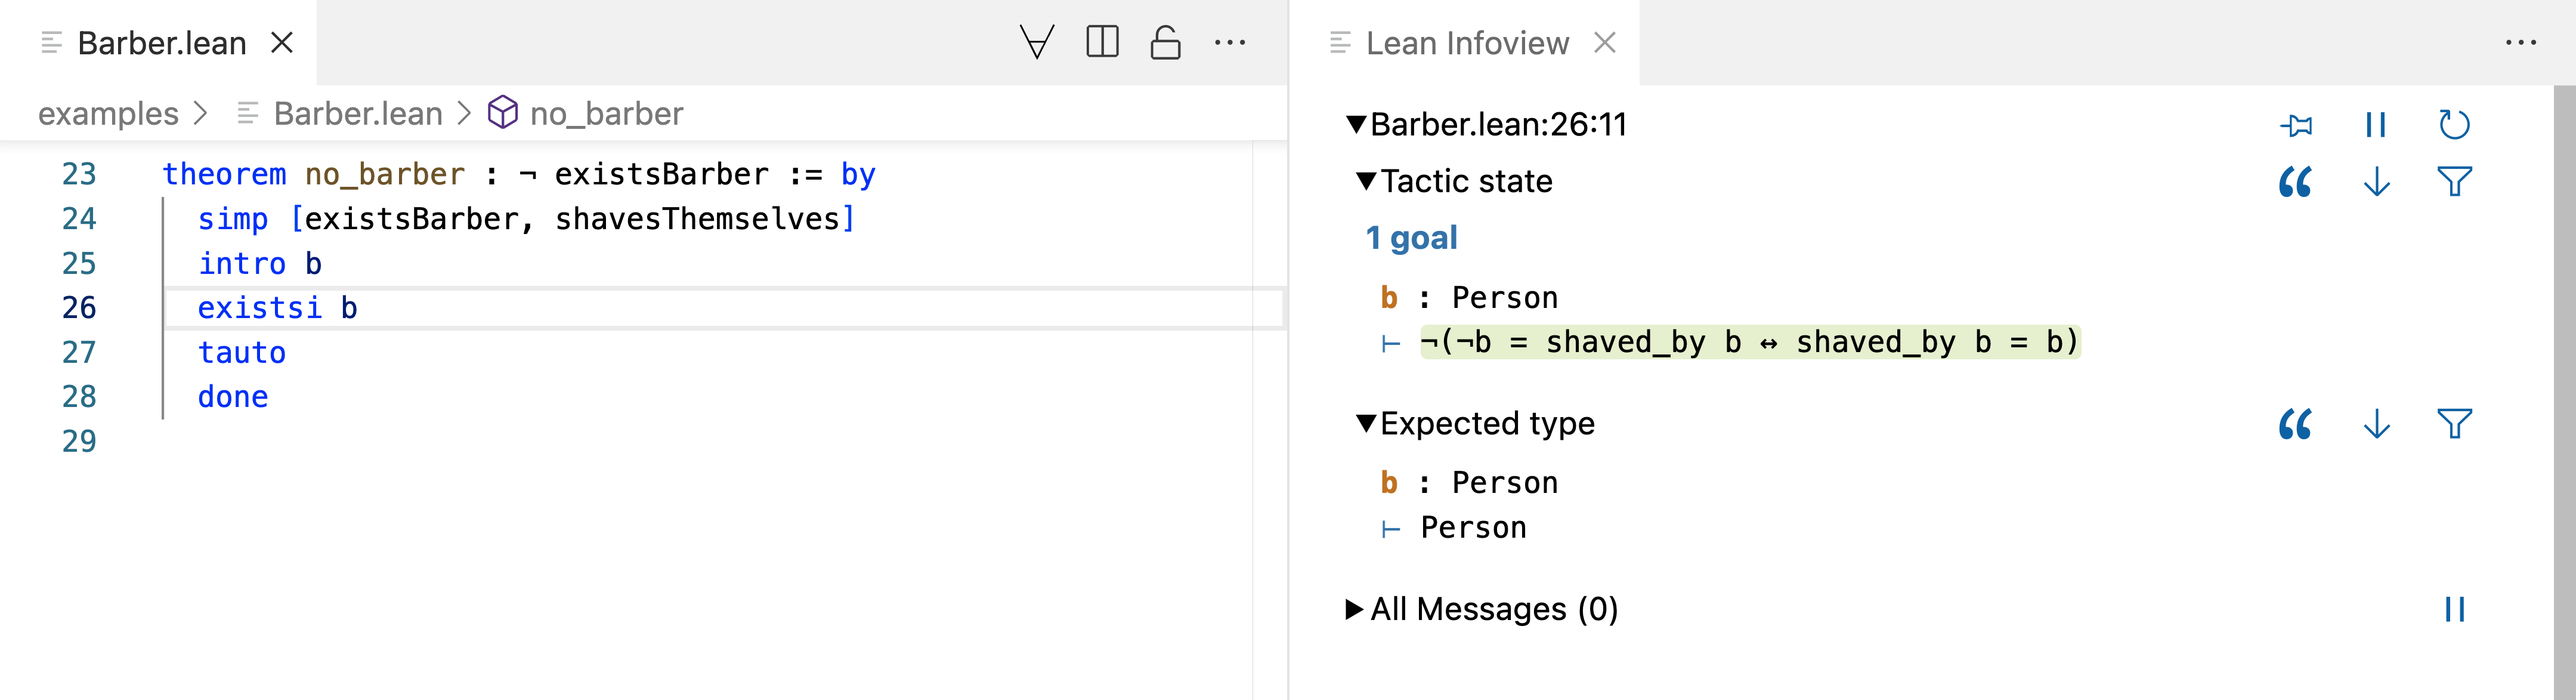
\includegraphics[width=\textwidth-1pt,trim={0 0 0 0},clip]{images/screenshots/barber-proof.png}}
  \caption{The proof of the nonexistence of a barber in the barber paradox, in Lean. The interactive proof state is on the right with the proof source on the left. }
  \label{fig:barber-proof}
\end{figure}

On line 25, we use the \texttt{simp} tactic (or we can also use \texttt{simp only}) to rewrite our Forge-defined predicates \texttt{existsBarber} and \texttt{shavesThemselves}. Due to the simplicity of the remaining goal (it is entirely in propositional logic), it can be closed using the \texttt{tauto} (tautology) tactic which repeatedly breaks down assumptions and splits goals with with logical connectives until it can close the goal. Full tactic states at each step of this proof are provided in \cref{appendix:barber-proof}. 

While simple, this example demonstrates the expressiveness of Forge programs embedded in Lean and the relative ease with which some proofs of translated properties can be executed. The following section, \cref{sec:mutex}, presents a more elaborative example of \textsc{Lforge}.

\subsection{A Mutual-Exclusion Protocol}\label{sec:mutex}

Here, we present a more comprehensive example that showcases more of the functionalities of \textsc{Lforge} and hopefully motivates real-world use cases of our tool. We model a basic mutual exclusion (mutex) protocol based on one of the examples presented in CSCI 1710 Logic for Systems \cite{l4s}. In the course, the example is posed with 2 competing processes over a mutex. Empowered with \textsc{Lforge}, we expand the model to include any number of processes. 

The example model contains \texttt{State} sigs that encapsulate the state of the entire system. Processes can have several states, \texttt{Uninterested}, \texttt{Waiting} (interested but not in critical state), \texttt{InCS} (in critical state). Each state contains a set of processes that have a flag raised demonstrating they are potentially interested in mutex. State transitions are modeled using predicates of the form
\begin{forge*}
pred transition[pre: State, p: Process, post: State] { ... }
\end{forge*}

Processes have 4 transitions: 
\begin{enumerate}
  \item \texttt{raise}: they can transitions from \texttt{Uninterested} to \texttt{Waiting} by raising their flag;
  \item \texttt{enter}: they can transition from \texttt{Waiting} to \texttt{InCS} provided they are the only flag raised;
  \item \texttt{lower}: if there is more than one flag raised, they can transition from \texttt{Waiting} back to \texttt{Uninterested} by lowering the flag;
  \item \texttt{leave}: they can transition from \texttt{InCS} to \texttt{Uninterested} when processes are done, lowering the flag. 
\end{enumerate}

We define a \texttt{good} predicate that states an invariant of our model that we wish to be true. In our case, the \texttt{good} predicate stipulates no two processes can be in the critical state (have acquired the lock) on the mutex at the same time, and any process that is waiting or in a critical state has a `flag' raised. We define an \texttt{init} state predicate that states all processes are in a state of \texttt{Uninterested} and no flags are raised. A predicate titled \texttt{properties} (users sometimes use the convention \texttt{traces}) encapsulates all properties of our system: that the initial state is good and for all pairs $\langle\texttt{pre}, \texttt{post}\rangle$ for which there is a transition between, $\texttt{pre}$ being a good state implies $\texttt{post}$ is a good state. This is to say, $\texttt{good}$ is an invariant property given our transition rules. 

To test our model and that it indeed has such desired properties, we can first run Forge on the test \texttt{properties is theorem} to check that Forge cannot find any counterexamples within its specified bounds. Then, as a next step, we can declare a theorem that states \texttt{properties} in Lean and prove our theorem. 

To prove \texttt{properties}, we can split up our property into the base case (proving that the \texttt{init} state is \texttt{good}) and that each of the 4 transitions preserves \texttt{properties}. We prove each transition separately in lemmas. 

An example of the tactic state during one of the proofs of one such lemma is showcased in \cref{fig:mutex-proof}. We note that the tactic state in \cref{fig:mutex-proof} represents a typical Lean proof state and what a user might encounter while using \textsc{Lforge} and Lean to prove specification properties, as opposed to our comically short proof in \cref{fig:barber-proof}. 

\begin{figure}[!htb]
  \centering
  \fbox{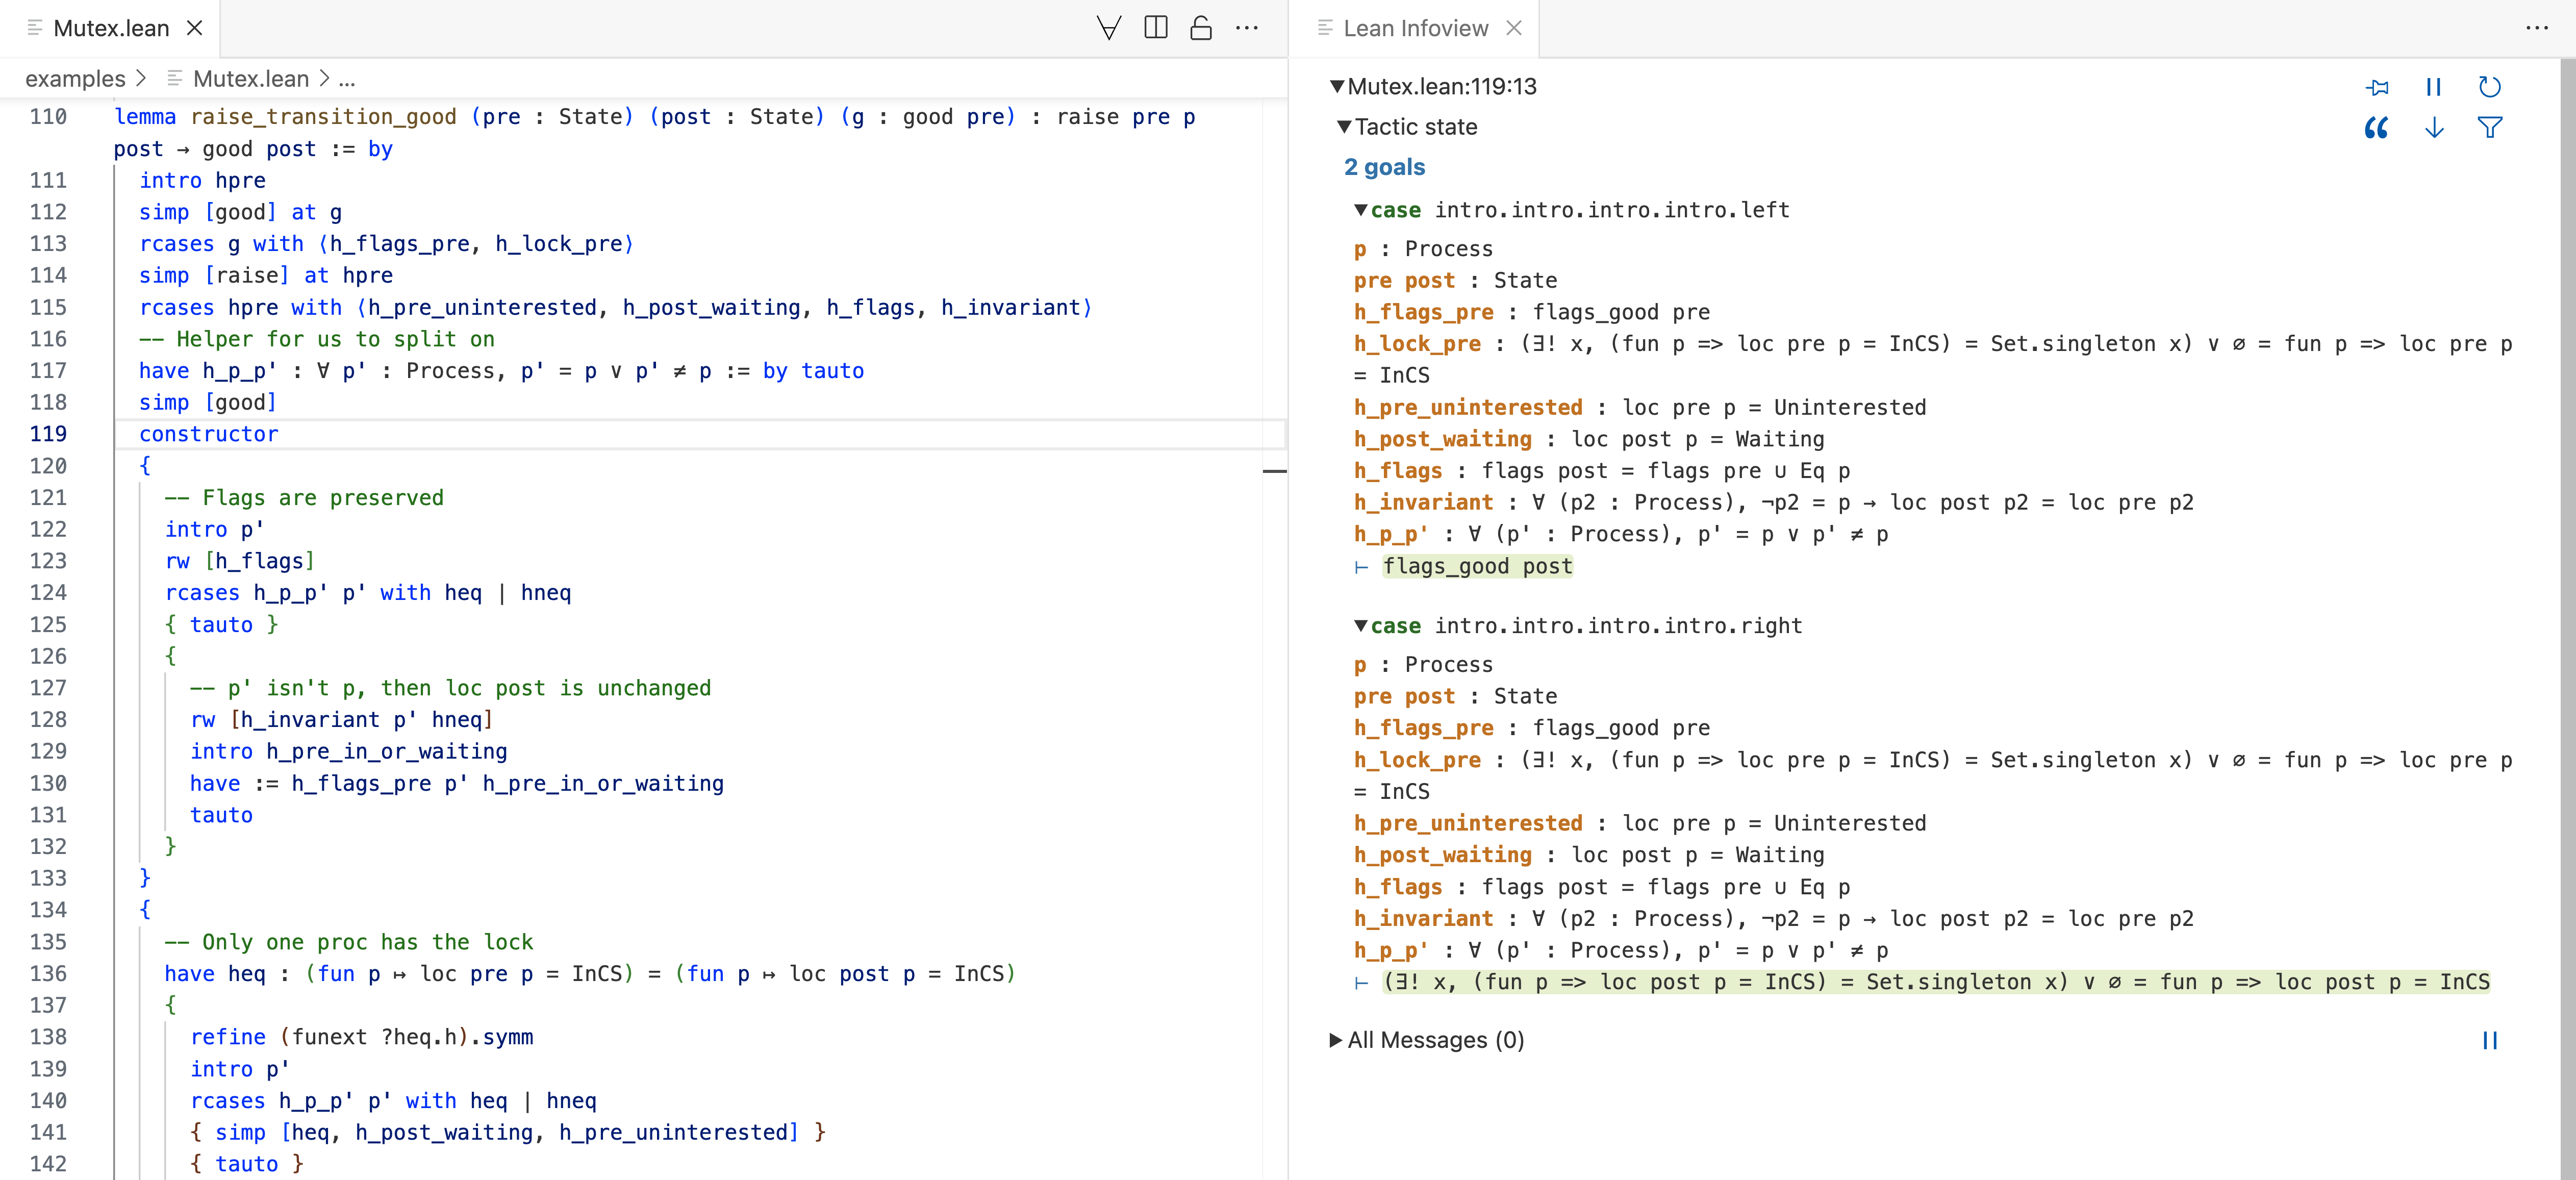
\includegraphics[width=\textwidth-1pt,trim={0 0 0 0},clip]{images/screenshots/mutex-proof.png}}
  \caption{The Lean tactic state at one line of our mutex proof that the \texttt{raise} transition is sound. }
  \label{fig:mutex-proof}
\end{figure}

\newpage

However, the proof was not without friction. Throughout the proof, dealing with sets was by far the most difficult. While Forge defaults to sets and `relations' as its primary type (see \cref{sec:everything-is-a-set}), Lean prefers expressions that are objects. This meant that proving statements like 
\begin{lean*}
{ x | x = p } = { p' } → p = p'
\end{lean*}
were unfortunately more difficult than necessary. An area of exploration and further work is to develop a library of theorems, lemmas, and tactics that specifically aid in proving Forge `set-style' statements within Forge. 

For a rough reference of length, our specification is roughly 70 lines long and our proof is roughly 250 lines long, which is standard for each. Neither the specification nor proof lengths were more involved than had they been solely in Forge or Lean respectively. The full source of this example is detailed in \cref{appendix:mutex-proof}. 

\subsection{Further Examples}
We provide three further examples (without proofs), to illustrate \textsc{Lforge}'s translation capabilities. Said examples translate fully using \textsc{Lforge} without any type errors. 

From the Logic for Systems course \cite{l4s}, we adapt the first Forge assignment on family trees, as well as the in-class example with a Tic-Tac-Toe board. Our examples are minimally modified specifications from the course and demonstrate \textsc{Lforge}'s capabilities of working with existing Forge specifications with little to no modification. 

Additionally, inspired by a research project that uses Forge to model distributed systems algorithms \cite{distributedforge}, we also model the two-phase atomic commitment protocol. Our example is an entirely new Forge specification that takes inspiration from this existing research. This serves as a more complex example of a system that might be valuable to be modeled in Forge and proven in Lean. 

The sources of said examples are referenced and specified further in \cref{appendix:additional-examples}. 